%%%%%%%%%%%%%%%%%%%%%%%%%%%%%%%%%%%%%%%%%
% Masters/Doctoral Thesis 
% LaTeX Template
% Version 2.2 (21/11/15)
%
% This template has been downloaded from:
% http://www.LaTeXTemplates.com
%
% Version 2.x major modifications by:
% Vel (vel@latextemplates.com)
%
% This template is based on a template by:
% Steve Gunn (http://users.ecs.soton.ac.uk/srg/softwaretools/document/templates/)
% Sunil Patel (http://www.sunilpatel.co.uk/thesis-template/)
%
% Template license:
% CC BY-NC-SA 3.0 (http://creativecommons.org/licenses/by-nc-sa/3.0/)
%
%%%%%%%%%%%%%%%%%%%%%%%%%%%%%%%%%%%%%%%%%

%----------------------------------------------------------------------------------------
%	PACKAGES AND OTHER DOCUMENT CONFIGURATIONS
%----------------------------------------------------------------------------------------

\documentclass[
11pt, % The default document font size, options: 10pt, 11pt, 12pt
oneside, % Two side (alternating margins) for binding by default, uncomment to switch to one side
english, % ngerman for German
singlespacing, % Single line spacing, alternatives: onehalfspacing or doublespacing
%draft, % Uncomment to enable draft mode (no pictures, no links, overfull hboxes indicated)
%nolistspacing, % If the document is onehalfspacing or doublespacing, uncomment this to set spacing in lists to single
%liststotoc, % Uncomment to add the list of figures/tables/etc to the table of contents
%toctotoc, % Uncomment to add the main table of contents to the table of contents
%parskip, % Uncomment to add space between paragraphs
%nohyperref, % Uncomment to not load the hyperref package
headsepline, % Uncomment to get a line under the header
]{MastersDoctoralThesis} % The class file specifying the document structure

\usepackage[utf8]{inputenc} % Required for inputting international characters
\usepackage[T1]{fontenc} % Output font encoding for international characters
\usepackage{amsmath,amssymb}
\usepackage{algorithm}
\usepackage{algpseudocode}


\usepackage{palatino} % Use the Palatino font by default
\usepackage{float} %force position of figures
\usepackage{wrapfig} %for wrapping images
\usepackage{longtable} %for creating tables across several pages
\usepackage{tabu} %for creating long tables
\usepackage{booktabs}
\usepackage{graphicx}
\usepackage[table,xcdraw]{xcolor}
\usepackage{cleveref}



\usepackage[backend=bibtex,style=ieee,maxcitenames=3,natbib=true]{biblatex} % User the bibtex backend with the authoryear citation style (which resembles APA)
\addbibresource{kilder.bib} % The filename of the bibliography

\usepackage[autostyle=true]{csquotes} % Required to generate language-dependent quotes in the bibliography

\usepackage[xindy, acronym, toc]{glossaries}
\usepackage{todonotes}

%%CUSTOM USE PACKAGES NOT FROM TEMPLATE
\usepackage{enumitem} %% USED FOR NO SPACE BETWEEN BULLET POINTS (DESIGN SECTION)
\usepackage{scrextend}
\usepackage{tabto}

\usepackage{verbatim}

\nocite{*}

%%USED TO DISPLAY CODE

\definecolor{pblue}{rgb}{0.13,0.13,1}
\definecolor{pgreen}{rgb}{0,0.5,0}
\definecolor{pred}{rgb}{0.9,0,0}
\definecolor{pgrey}{rgb}{0.46,0.45,0.48}
\definecolor{lightb}{RGB}{217,224,250}
\definecolor{SDUblue}{RGB}{1,67,128}

\usepackage{listings}
\lstset{language=Java,
  showspaces=false,
  showtabs=false,
  breaklines=true,
  showstringspaces=false,
  breakatwhitespace=true,
  commentstyle=\color{pgreen},
  keywordstyle=\color{pblue},
  stringstyle=\color{pred},
  basicstyle=\ttfamily,
  moredelim=[il][\textcolor{pgrey}],
  moredelim=[is][\textcolor{pgrey}]{\%\%}{\%\%}
}


\makeglossaries
	
%%!TEX root=../main.tex

%%%%%%%%%%% GLOSSARY ENTRIES %%%%%%%%%%%
\newglossaryentry{NoSQL}
{
	name=\textit{No-SQL},
	plural=\textit{No-SQL},
	description={Not Only SQL: a database which relies on collections and documents rather than the classical relational databases with tables, columns and rows}
}

\newglossaryentry{Struct}
{
	name=\textit{Struct A/S},
	plural=\textit{Struct A/S},
	description={A company specializing in E-commerce solutions for businesses Struct has partnered with the project group and supplied the data for this Bachelor project}
}

\newglossaryentry{MongoDB}
{
	name=\textit{MongoDB},
	plural=\textit{MongoDB},
	description={A No-SQL database implementation}
}

\newglossaryentry{Amazon}
{
	name=\textit{Amazon},
	plural=\textit{Amazon},
	description={Amazon is a retail giant selling product to consumers in many different categories}
}

\newglossaryentry{EC2Instance}
{
	name=\textit{EC2 Instance},
	plural=\textit{EC2 Instances},
	description={A linux based virtual server running in the AWS cloud}
}

\newglossaryentry{ecommerce}
{
	name=\textit{e-commerce},
	plural=\textit{e-commerces},
	description={The business of buying and selling online}
}

\newglossaryentry{datamining}
{
	name=\textit{datamining},
	description={An analysis technique trying to discover useful information and relationships in large amounts of existing data}
}

\newglossaryentry{gls-API}
{
	name=\textit{API},
	description={An interface designed to integrate one piece of software with another}
}

\newglossaryentry{contentbased}
{
	name=\textit{Content-based filtering},
	description={A recommendation technique focusing on the content (description) of an item and how it relates to other items}
}

\newglossaryentry{knowledgebased}
{
	name=\textit{Knowledge-based recommendations},
	description={A recommendation technique relying on deep knowledge about the offered items}
}

\newglossaryentry{collaborativefiltering}
{
	name=\textit{Collaborative filtering},
	description={A recommendation technique linking items and users based on user-behavior, item descriptions etc.}
}

\newglossaryentry{hybrid}
{
	name=\textit{Hybrid recommendations},
	description={A mix of other recommendation techniques such is \gls{contentbased}, \gls{knowledgebased} and \gls{collaborativefiltering}}
}

\newglossaryentry{aspnet}
{
	name=\textit{ASP.NET Core},
	description={Open-source and cross-platform framework for building modern internet connected applications. It consists of modular components with minimal overhead to retain flexibility when constructing solutions}
}

\newglossaryentry{gls-REST}
{
	name=\textit{REST},
	description={An architectural style used for communication across systems on the internet}
}

\newglossaryentry{Docker}
{
	name=\textit{Docker},
	description={Docker is an open-source project that automates the deployment of applications inside software containers}
}

\newglossaryentry{amazonwebservice}
{
	name=\textit{Amazon Web-services},
	description={Provides on-demand cloud computing platforms}
}

\newglossaryentry{DockerContainer}
{
	name=\textit{Docker container},
	description={A lightweight stand-alone executable package of a piece of software that includes everything needed to run it}
}




%%%%%%%%%%% ACRONYMS %%%%%%%%%%%

\newacronym{DTO}{\textit{DTO}}{Data transfer object}

\newacronym[see={[Glossary:]{gls-API}}]{API}{\textit{API}}{Application Programming Interface\glsadd{gls-API}}

\newacronym[see={[Glossary:]{gls-REST}}]{REST}{\textit{REST}}{REpresentational State Transfer\glsadd{gls-REST}}

\newacronym{HTTP}{\textit{HTTP}}{HyperText Transfer Protocol}

\newacronym{XML}{\textit{XML}}{Extensible Markup Language}




%----------------------------------------------------------------------------------------
%	MARGIN SETTINGS
%----------------------------------------------------------------------------------------

\geometry{
	paper=a4paper, % Change to letterpaper for US letter
	inner=1.5cm, % Inner margin
	outer=1.5cm, % Outer margin
	bindingoffset=1cm, % Binding offset
	top=1.5cm, % Top margin
	bottom=1.5cm, % Bottom margin
	%showframe,% show how the type block is set on the page
}

%----------------------------------------------------------------------------------------
%	THESIS INFORMATION
%----------------------------------------------------------------------------------------

\thesistitle{Datamining and its use} % Your thesis title, this is used in the title and abstract, print it elsewhere with \ttitle
\supervisor{Jan Corfixen Sørensen \textsc{Sørensen}} % Your supervisor's name, this is used in the title page, print it elsewhere with \supname
\examiner{} % Your examiner's name, this is not currently used anywhere in the template, print it elsewhere with \examname
\degree{Software Engineering 6. semester} % Your degree name, this is used in the title page and abstract, print it elsewhere with \degreename
\author{Lasse Bjørn \textsc{Hansen}\\
	Simon \textsc{Flensted}} % Your name, this is used in the title page and abstract, print it elsewhere with \authorname
\addresses{} % Your address, this is not currently used anywhere in the template, print it elsewhere with \addressname

\subject{Software Engineering} % Your subject area, this is not currently used anywhere in the template, print it elsewhere with \subjectname
\keywords{} % Keywords for your thesis, this is not currently used anywhere in the template, print it elsewhere with \keywordnames
\university{University of Southern Denmark} % Your university's name and URL, this is used in the title page and abstract, print it elsewhere with \univname
\department{TEK} % Your department's name and URL, this is used in the title page and abstract, print it elsewhere with \deptname
\group{Group ??} % Your research group's name and URL, this is used in the title page, print it elsewhere with \groupname
\faculty{TEK - Mærsk McKinney Møller Institut} % Your faculty's name and URL, this is used in the title page and abstract, print it elsewhere with \facname

\hypersetup{pdftitle=\ttitle} % Set the PDF's title to your title
\hypersetup{pdfauthor=\authorname} % Set the PDF's author to your name
\hypersetup{pdfkeywords=\keywordnames} % Set the PDF's keywords to your keywords

\begin{document}

\frontmatter % Use roman page numbering style (i, ii, iii, iv...) for the pre-content pages

\pagestyle{plain} % Default to the plain heading style until the thesis style is called for the body content

%----------------------------------------------------------------------------------------
%	TITLE PAGE
%----------------------------------------------------------------------------------------

\begin{titlepage}
\begin{center}

\textsc{\LARGE \univname}\\[1.5cm] % University name
\textsc{\Large Software Engineering 6. Semester}\\[0.5cm] % Thesis type

\HRule \\[0.4cm] % Horizontal line
{\huge \bfseries \ttitle}\\[0.4cm] % Thesis title
\HRule \\[1.5cm] % Horizontal line
 
\begin{minipage}{0.4\textwidth}
\begin{flushleft} \large
\emph{Author:}\\
\authorname % Author name - remove the \href bracket to remove the link
\end{flushleft}
\end{minipage}
\begin{minipage}{0.4\textwidth}
\begin{flushright} \large
\emph{Supervisor:} \\
{\supname} % Supervisor name - remove the \href bracket to remove the link  
\end{flushright}
\end{minipage}\\[3cm]

\includegraphics{SDU-Logo} % University/department logo - uncomment to place it
\large \textit{A report submitted in fulfillment of the requirements\\  of \degreename}\\[0.3cm] % University requirement text
\textit{at}\\[0.4cm]
\univname\\\deptname\\[2cm] % Research group name and department name
 
{\large \today}\\[4cm] % Date

 
\vfill
\end{center}
\end{titlepage}

%----------------------------------------------------------------------------------------
%	ABSTRACT PAGE
%----------------------------------------------------------------------------------------

%\thispagestyle{plain}

%\chapter{Abstract}
\textit{Datamining has become a growing part of modern software solutions. In the business of e-commerce, companies have realized how important prober analysis and organization of data can be to increase sales. Once data is organized in a desirable manner, companies can exploit the data to learn more about their customers.\\
This paper describes the initial datamining of a large datadump, a system for maintaining the data and an algorithm that provides tailored product recommendations to visitors of a webshop.
The development of the algorithm is inspired by similar existing systems, among these the retail giant Amazon. The final product is designed according to the requirements acquired from the collaborating company Struct A/S.}
\clearpage

%----------------------------------------------------------------------------------------
%	PREFACE / ACKNOWLEDGMENTS
%----------------------------------------------------------------------------------------

%\chapter{Preface}
This report has been written by Lasse Bjørn Hansen and Simon Haugaard Flensted. It is the documented result of a bachelor project at the 6th semester of Software Engineering at University of Southern
Denmark in Odense (01/02/2017 - 22/05/2017). The report documents the implementation and the final product of the project.\\

\noindent We would like to thank our bachelor supervisor Jan Corfixen Sørensen for guiding, being available and helping throughout the project. We would also like to thank the company \gls{Struct}, especially Peter Melchiorsen and Simon Lyder for providing the case that formed the foundation of the project, and providing continuous feedback. At last the group would like to thank Casper Middelhede and Lars Bo Meixner for reading through this report and providing valuable feedback.
\\

\noindent This report was handed in May 22, 2017.
\\
\\
\\

\noindent\rule[0.5em]{26em}{0.5pt}\\
\noindent Lasse Bjørn Hansen \tab 64753953
\\
\\

\noindent\rule[0.5em]{26em}{0.5pt}\\
\noindent Simon Haugaard Flensted \tab 409994
\\
\\

%----------------------------------------------------------------------------------------
%	QUOTATION PAGE
%----------------------------------------------------------------------------------------

\vspace*{0.2\textheight}

\noindent\Huge{\enquote{\itshape Some quote}}\bigbreak
\hfill \Large{- Gruppe 3}
\normalsize

%----------------------------------------------------------------------------------------
%	READING GUIDE
%----------------------------------------------------------------------------------------

\thispagestyle{plain}
%\include{Chapters/Reading-guide}
%----------------------------------------------------------------------------------------
%	LIST OF CONTENTS/FIGURES/TABLES PAGES
%----------------------------------------------------------------------------------------

\tableofcontents % Prints the main table of contents
\clearpage

%----------------------------------------------------------------------------------------
%	EDITORIAL
%----------------------------------------------------------------------------------------

%\thispagestyle{plain}


%----------------------------------------------------------------------------------------
%	GLOSSARY LIST
%----------------------------------------------------------------------------------------

\printglossaries

%----------------------------------------------------------------------------------------
%	THESIS CONTENT - CHAPTERS
%----------------------------------------------------------------------------------------

\mainmatter % Begin numeric (1,2,3...) page numbering

\pagestyle{thesis} % Return the page headers back to the "thesis" style

% Include the chapters of the thesis as separate files from the Chapters folder
% Uncomment the lines as you write the chapters
% Chapter Template

\chapter{Introduction} % Main chapter title

\label{ChapterX} % Change X to a consecutive number; for referencing this chapter elsewhere, use \ref{ChapterX}

%----------------------------------------------------------------------------------------
%	SECTION 1
%----------------------------------------------------------------------------------------

This chapter covers the motivation behind the project and important areas relating to the project. It introduces the collaborating company who helped provide a case, data, and feedback. Finally the scope of the project is defined.

\section{Motivation}
The amount of data being processed on the server side and within large systems is continuously increasing. This data should be structured and modeled in a way that makes it easily accessible and easy to work with. Handling large amounts of data the right way can prove to be very useful, not only to the company who possesses the data, but also to the end users of a product. \Gls{datamining} is very useful in order to achieve this.
The company Struct A/S has provided a software engineering task of creating product recommendations where data mining will create the foundation. This report will address the use of data mining, the development of a solution that provides the user with intelligent product recommendations, and makes it possible to maintain current and future data.

\subsection{Data mining}
Data mining is an analysis technique trying to discover useful information and relationships in large amounts of existing data \cite{dataminingSource}. \\  
Data mining has become an important part of modern software engineering. Lots of companies tends to store large amount of data. If the data is analyzed properly and put to use, it can add tremendous value to the company as well as its users. In this case \gls{Struct} has stored information about users visiting one of their customers webshops. Previously, this data was stored in a database not optimized for product recommendations and not put to use. By processing the data properly, using data mining, it can be structured in a way that makes it useful to the company e.g. product recommendations.

\color{black}
\subsection{Product recommendation}
If an e-commerce company wants to increase its profit, product recommendation has proven to be very beneficial \cite{BigCommerce}. This is heavily used by multiple companies including the retail giant Amazon\cite{Fortune}. If you can predict what products your costumer may find useful, additional sales become more frequent. A data set like the one provided by Struct A/S, can make it possible to predict customer needs.

\section{Struct A/S}
Struct A/S is an IT-company specializing in developing E-commerce solutions such as web shops and Product Information Management systems. The customers of Struct A/S are the web shop owners. Struct A/S has provided a data set from one of these customers containing information about the visitors of their web shop \cite{Struct}.


\section{Scope}
Product recommendation and data mining are massive subjects consisting of much literature. Many large companies have tackled the challenge of providing recommendations for their users and spent a lot of time perfecting their algorithms.\\
This project will focus on designing and implementing a product recommendation algorithm capable of providing "good recommendations" The term "good recommendations" is a very loose term because it can vary from business to business or even from individual to individual. To directly compare the developed algorithm to others on the market would require access to these algorithms as well as a test on the same data. This has not been possible to acquire and therefore no direct comparison will be made. \\
In the limited time of this project it is not reasonable to expect Struct A/S to be able to begin using the API which means no online validation can be made. \\
The project comes with limited funds and as a result of this, some less optimal but free alternatives have been used for hosting the algorithm. \\
Only the requirements necessary to have a functional product are implemented as there is ample material to focus on.

% Chapter Template

\chapter{Problem statement} % Main chapter title

\label{Chapter1} % Change X to a consecutive number; for referencing this chapter elsewhere, use \ref{ChapterX}

%----------------------------------------------------------------------------------------
%	SECTION 1
%----------------------------------------------------------------------------------------

\section{Problem description}

The initial problem/challenge  is given to us by the company Struct A/S and is described as follows: \\\\
When launching sites, whether it being regular websites or web shops, a lot of user activity is logged. We therefore have a large amount of data associated with each of our sites but do not currently use it. \\
In the future we would like to be able to use logged data to generate an insight into the user activity on our site and actively use this data to create a personalized experience for the users. \\\\

This project will handle the initial normalization of the data, storing it in a scalable way and utilizing the data to create features which add value for the users. In order to achieve this, theory has to become implementation. Research is required in terms of data storing, data mining and recommendation algorithms. This research is implemented in the end system creating an API allowing Struct A/S to get useful information from the data such as the recommended products for a certain user. This API will be the final product and will utilize different technologies and algorithms.





\section{Problem statement}
The data we have been given is in a de-normalized format and the problem therefore comes with two challenges - normalizing the data and utilizing the data to create a personalized experience for the users. \\
This leads to the following research questions:
\begin{itemize}
\item How can you effectively normalize large amounts of data?
\item How can you optimally store and access data in a scalable way?
\item How can you utilize the data to generate useful features for the end user?
\end{itemize}

% Chapter Template

\chapter{Requirements} % Main chapter title

\label{Chapter3} % Change X to a consecutive number; for referencing this chapter elsewhere, use \ref{ChapterX}

%----------------------------------------------------------------------------------------
%	SECTION 1
%----------------------------------------------------------------------------------------

\section{Requirements engineering}
The requirements of the project are categorized into functional and non-functional requirements. These requirements were derived from the original case given by Struct A/S (Appendix \ref{Case}), continuously planned meetings with Struct A/S and our supervisor, and as a part of the constant research done during the progress of the project. \\
The functionality of the final product fulfills the most important aspects of the case, and the requirements derived from the client meetings.

\subsection{Functional requirements} 
The most important features of the system includes delivery of good quality product recommendation and handling of new data. These are very complex features and a lot of requirements must be fulfilled in order to realize them. The most crucial functional requirements can be seen in table \ref{table:functionalrequirements}. These requirements have been the driving force throughout the project. For a complete list of functional requirements, see the git backlog \cite{ProductBacklog}.
\begin{table}[]
	\centering
		\begin{tabular}{l|l}
			\rowcolor[HTML]{96B1FF} 
			\multicolumn{1}{c|}{\cellcolor[HTML]{96B1FF}F01} & \begin{tabular}[c]{p{.9\textwidth}}\textbf{The webshop developer can provide tailored product recommendations to his customers.}\\ When the API is provided with information about a visitor, tailored recommendations to the customer must be returned. If the data about the visitor is insufficient to calculate enough tailored recommendations, the most popular products within the last 30 days must be used to present enough recommendations.\end{tabular} \\
			F02                                              & \begin{tabular}[c]{p{.9\textwidth}}\textbf{The webshop developer can store new behavior data for a visitor in the database.} \\ When the API is provided with the required information, new behavior data must be stored in the database.\end{tabular}                                                                                                                                                                                                              \\
			\rowcolor[HTML]{96B1FF} 
			F03                                              & \begin{tabular}[c]{p{.9\textwidth}}\textbf{The webshop developer can store new behavior data for a product in the database.} \\ When the API is provided with the required information, new behavior data must be stored in the database.\end{tabular}                                                                                                                                                                                                              \\
			F04                                              & \begin{tabular}[c]{p{.9\textwidth}}\textbf{The webshop developer can store new product groups in the database.} \\ When the API is provided with the required information, a new product group must be stored in the database.\end{tabular}                                                                                                                                                                                                                         \\
			\rowcolor[HTML]{96B1FF} 
			F05                                              & \begin{tabular}[c]{p{.9\textwidth}}\textbf{The webshop developer can store new visitors in the database.}\\ When the API is provided with the required information, a new visitor must be stored in the database.\end{tabular}                                                                                                                                                                                                                                      \\
			F06                                              & \begin{tabular}[c]{p{.9\textwidth}}\textbf{The webshop developer can store new products in the database.}\\ When the API is provided with the required information, a new product must be stored in the database.\end{tabular}   
			\\
			\rowcolor[HTML]{96B1FF} 
			F07                                              & \begin{tabular}[c]{p{.9\textwidth}}\textbf{The webshop developer can update existing product groups in the database.}\\ When the API is provided with the required information, a product group should be updated.\end{tabular}   
			\\
			F08                                              & \begin{tabular}[c]{p{.9\textwidth}}\textbf{The webshop developer can update existing products in the database.}\\ When the API is provided with the required information, a product should be updated.\end{tabular}        
			\\
			\rowcolor[HTML]{96B1FF} 
			F09                                              & \begin{tabular}[c]{p{.9\textwidth}}\textbf{The webshop developer can update a visitor in the database.}\\ When the API is provided with the required information, the visitor should be updated.\end{tabular}   
			\\
			F10                                              & \begin{tabular}[c]{p{.9\textwidth}}\textbf{The webshop developer can delete existing behavior in the database.}\\ When the API is provided with the required information, behavior data should be deleted in order to keep the data up-to-date.\end{tabular}     
			\\
			\rowcolor[HTML]{96B1FF} 
			F11                                              & \begin{tabular}[c]{p{.9\textwidth}}\textbf{The webshop developer can delete an existing visitor in the database.}\\ When the API is provided with the required information, the visitor should be deleted in order to keep the data up-to-date.\end{tabular}     
			\\
			F12                                              & \begin{tabular}[c]{p{.9\textwidth}}\textbf{The webshop developer can delete an existing product group in the database.}\\ When the API is provided with the required information, the product group should be deleted in order to keep the data up-to-date.\end{tabular}    
			\\
			\rowcolor[HTML]{96B1FF} 
			F13                                              & \begin{tabular}[c]{p{.9\textwidth}}\textbf{The webshop developer can delete an existing product in the database.}\\ When the API is provided with the required information, the product should be deleted in order to keep the data up-to-date.\end{tabular}     
			\\
			F14                                              & \begin{tabular}[c]{p{.9\textwidth}}\textbf{The The webshop developer can store new order data for an order in the database.} \\ When the API is provided with the required information, new order data must be stored in the database.\end{tabular}   
			\\   
			\rowcolor[HTML]{96B1FF} 
			F15                                              & \begin{tabular}[c]{p{.9\textwidth}}\textbf{The webshop developer can delete an existing order in the database.}\\ When the API is provided with the required information, the order should be deleted in order to keep the data up-to-date.\end{tabular}                                                      
		\end{tabular}%
	\caption{Functional requirements}
	\label{table:functionalrequirements}
\end{table}

As seen in table \ref{table:functionalrequirements}, the functional requirements of the final product can be compressed into 15 requirements. This corresponds with the wish of a simple API, that provides good quality product recommendations. F01 - \textit{provide recommendations}, was the most important requirement and has therefore acted as an ongoing task during the entire development of the product. F02-F15 were secondary requirements as they were not crucial before the recommendation algorithm was implemented. Once the algorithm was developed, the remaining functional requirements were needed to keep the data updated.

\subsection{Non-functional requirements}
The non-functional requirements were described at an early stage, and later clarified at the planned meetings. The non-functional requirements can be seen in table \ref{table:nonfunctionalrequirements}.

\begin{table}[]
	\centering
	\begin{tabular}{l|l}
		\rowcolor[HTML]{96B1FF} 
		\multicolumn{1}{c|}{\cellcolor[HTML]{96B1FF}NF01} & \begin{tabular}[c]{p{.9\textwidth}}\textbf{Programming language and platform}\\The API should be developed in C\# .NET core.\end{tabular} \\
		NF02                                              & \begin{tabular}[c]{p{.9\textwidth}}\textbf{Efficiency}\\ Recommendations must be delivered within 40ms. \end{tabular}                                                                                                                                                                                                              \\
		\rowcolor[HTML]{96B1FF} 
		NF03                                              & \begin{tabular}[c]{p{.9\textwidth}}\textbf{Scalability}\\The data used for product recommendations should be stored in a fitting scalable No-SQL database. \end{tabular}                                                                                                                                                                                                              \\
		NF04                                              & \begin{tabular}[c]{p{.9\textwidth}}\textbf{Accessibility}\\The API should be easy accessible through a web service. \end{tabular}                                                                                                                                                                                                                                                                                                                                                                                                                                          
	\end{tabular}%
	\caption{Non-functional requirements}
	\label{table:nonfunctionalrequirements}
\end{table}

Few non-functional requirements were discovered, but these turned out to be challenging to accommodate. The platform Struct use as the main tool for developing is based on the programming language C\#. As a result of this, NF01 was derived. Net core was chosen because of its high performance and scalable systems, which was needed to realize NF02 - \textit{Recommendations must be delivered within 40ms}.\cite{NetCore}
NF02 was probably the most challenging requirement to fulfill, however very important since a fast responding website is imperative. At the beginning Struct had a wish that the new database for recommendation data had to be scalable up to billions of records. Because of the denormalized data structure, it was agreed that a No-SQL database would be the right approach \cite{NoSQLScalability}. This resulted in requirement NF03 - \textit{Data should be stored in a scalable No-SQL database}. In order to lower the amount of effort needed to integrate the recommendation system, the API had to easily accessible and the data output had to be in a standardized format. This resulted in requirement NF04 - \textit{The API should be easy accessible through a web service}.

%!TEX root=../main.tex
% Chapter Template

\chapter{Design} % Main chapter title

\label{Chapter3} % Change X to a consecutive number; for referencing this chapter elsewhere, use \ref{ChapterX}

%----------------------------------------------------------------------------------------
%	SECTION 1
%----------------------------------------------------------------------------------------

\section{Conceptual overview of the system}
The system is developed as a part of the classic architectural pattern, Model-View-Controller (MVC) \ref{PatternsOfEnterprise}. The system itself consists of the Model and Controller part, and lets the client be responsible for the view, which in this case is the web shop. Figure \ref{fig:MVC} shows how the system is layered. Data is sent to the controller which simply communicates the data between the logic (model) of the system and the view. The logic (model) is responsible for communication with the database, calculations regarding product recommendations, and handling new incoming data. The persistance layer is part of the model as described in \cite{PatternsOfEnterprise}  \textit{"When you're working with a model you are thinking about business policies, perhaps database interactions."}.

\begin{figure}[H]
	\centering
	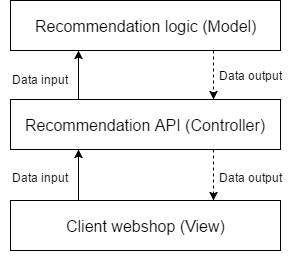
\includegraphics[width=.4\linewidth]{Figures/MVC.png}
	\caption{The Model-View-Controller (MVC) pattern applied on the system}
	\label{fig:MVC}
\end{figure}

\subsection{Recommendation API (Controller)}
The recommendation system is designed according to the MVC pattern described above. The controller layer takes input from the user (the web shop) and passes the information to the model layer. The model layer consists of the objects seen in the domain model in Chapter \ref{analysis} as well as classes for handling the business logic and persistence. The different layers communicate through interfaces in order to be able to substitute implementations in the future. \\
The controller layer is split into two classes, one for handling when the user requests recommendations which relates to functional requirement NF01 and another for handling the data coming from the web shops relating to functional requirements F02-F15.


\subsection{Recommendation logic (Model)}
The recommendation logic is where the main operations of the system takes place. The model layer consists of five packages, and is made accessible to the controller layer through three interfaces. All classes used for calculations are placed in the Business package. This is where the product recommendations are calculated before being sent back to the control layer. This is also the package where any offline-calculation is made before it is stored in the database. The persistence package handles all information that needs to be communicated with the database. The Entities and Utility package creates an easier and more manageable way of communicating data around within the model layer. All communication between the Controller-layer and the Model-layer is done through the interfaces seen in the Communication package. These interfaces are implemented by their corresponding classes in the Business and Persistence packages. The implementation of the Model-layer is discussed further in Chapter \ref{Chapter5}. \\
A package diagram of the Controller and Model layer can be seen in figure \ref{fig:PackageDiagram}

\begin{figure}[H]
	\centering
	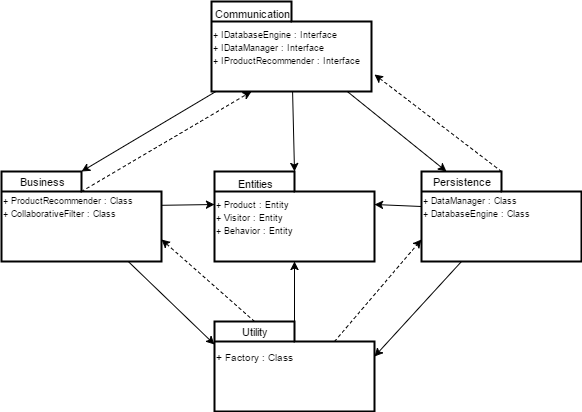
\includegraphics[width=.8\linewidth]{Figures/PackageDiagram.png}
	\caption{Package diagram of the model layer}
	\label{fig:PackageDiagram}
\end{figure}

\section{Client-Server}
When put to use, the recommendation system will be distributed and play the server role in a Client-Server model. The system should be considered an application solely for providing product recommendations. In this scenario, the client is the web shop that needs to provide recommendations to one of its users. The client is also able to ask the server to update its database or store new content in the database, but the concept is the same and just as simple as the request for product recommendations. The Client-Server model of the system can be seen in figure \ref{fig:ClientServer}

\begin{figure}[H]
	\centering
	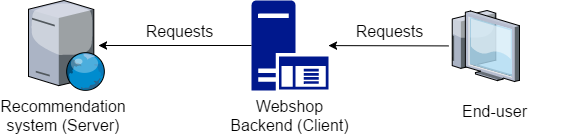
\includegraphics[width=.8\linewidth]{Figures/ClientServer.png}
	\caption{Package diagram of the model layer}
	\label{fig:ClientServer}
\end{figure}

\section{Database design}
Specific requirements for the storage of data was set by Struct, as they wanted a largely scalable structure of the data. The technology chosen was \gls{NoSQL}.
The data demands are not clearly specified in the beginning and with No-SQL it is easy to add or remove data or even change the data types on the fly whereas traditional relational databases have very strict data requirements, this also means that all data restrictions have to be handled in the code. No-SQL's denormalized format also allows for faster retrieval of a single item without having to do joins or complex SQL queries. Finally No-SQL is easier to scale across multiple servers and many engines have built in scaling functionalities \cite{SQLvsNOSQL} which can come in handy when multiple clients begin using the service. A downside of No-SQL compared to relational databases is the fact it does not focus much on Online Transaction Processing (OLTP) which means there is no guarantee that the data is always stored completely. Overall No-SQL is a good fit for this project since scalability and speed is imperative. \\\\

A brief overview of the different terminology for SQL and No-SQL is given in table \ref{sqlvsnosql_table}.
\begin{table}[H]
	\centering
	\caption{SQL vs No-SQL terminology}
	\label{sqlvsnosql_table}
	\begin{tabular}{|l|l|p{8cm}|}
		\hline
		\textbf{SQL}   & \textbf{No-SQL}     & \textbf{Comment}                                                                                                    \\ \hline
		Table & Collection &                                                                                                            \\ \hline
		Row   & Document   & A No-SQL document can contain more complex datatypes compared to a row in SQL e.g arrays or other documents \\
		\hline
	\end{tabular}
\end{table}

The database design mimics the domain model by representing real world concepts such as a Visitors and their Behavior and Products. The No-SQL design can be seen in figure \ref{documents}.

\begin{table}[H]
	\centering
	\caption{An overview of the fields in each document in the collections}
	\label{documents}
	\begin{tabular}{|l|l|p{7cm}|}
		\hline
		\textbf{Document} & \textbf{Fields}                                                                                                                          & \textbf{Comment}                                                                   \\ \hline
		Visitor           & \begin{tabular}[c]{@{}l@{}}Id: string\\ Behaviors: array\\ ProfileUID: string\\ CustomerUID: string\end{tabular}                         & The behavior array is an array of Behavior documents which contains all the behaviors of the specific visitor \\ \hline
		Product           & \begin{tabular}[c]{@{}l@{}}Id: int\\ ProductGroupId: int\\ VisitorId: stringArray\\ Description: string\\ Created: DateTime\end{tabular} &     The visitorId array contains Ids of all visitors who have looked at this product    \\ \hline
		Behavior & \begin{tabular}[c]{@{}l@{}}Type: string \\ Id: int \\ Timestamp: DateTime \end{tabular} & A behavior document holds information about a particular behavior \\ \hline
	\end{tabular}
\end{table}

An example of a Visitort document can be seen in figure \ref{visitorDoc} and an example of a Product document can be seen in appendix \ref{productDoc}.
\begin{figure}[H]
	\centering
	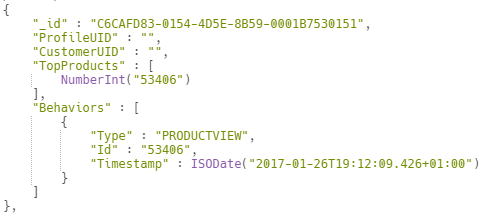
\includegraphics{visitorDocument}
	\caption{A Visitor document example}
	\label{visitorDoc}
\end{figure}

The topProducts array seen in Appendix \ref{productDoc} was not part of the original data transformation, but rather a part of the recommendation algorithm explained in Chapter \ref{Chapter5}.

%\include{Chapters/Chapter4}
%\include{Chapters/Chapter5} 
%\include{Chapters/Chapter6}
%\include{Chapters/Chapter7} 
%\include{Chapters/Conclusion}
%\include{Chapters/Chapter8}
%\include{Chapters/Chapter9}
%\include{Chapters/Chapter10}

%----------------------------------------------------------------------------------------
%	THESIS CONTENT - APPENDICES
%----------------------------------------------------------------------------------------

\appendix % Cue to tell LaTeX that the following "chapters" are Appendices
%\input{Appendices/Code-conventions}
%% Chapter Template

\chapter{Process} % Main chapter title

\label{Appendix D} % Change X to a consecutive number; for referencing this chapter elsewhere, use \ref{ChapterX}

%----------------------------------------------------------------------------------------
%	SECTION 1
%----------------------------------------------------------------------------------------

\section{Introduction}
This appendix elaborates on the process behind the development of the final product.

The project was initiated by the case presented by Struct A/S. The core of the case was as follows:
\textit{"When launching sites, whether it being regular websites or web shops, a lot of user activity is logged. We therefore have a large amount of data associated with each of our sites but do not currently use it.} \\
\textit{In the future we would like to be able to use logged data to generate an insight into the user activity on our site and actively use this data to create a personalized experience for the users."} \\
Eventually this case led to the problem statement seen in chapter \ref{Problem}.

A variety of technologies and methods was used throughout the realization of the product. To ensure that the process went as smooth as possible, the agile software development framework, Scrum, was used as a framework to structure and organize the work \cite{Scrum}.

\section{Scrum}
Scrum is the main pillar for controlling the process of the project. Since the developing team only consisted of two students, Scrum is not applied 100\% to the project. This section elaborates on the usage of Scrum and how the different roles were fulfilled.

\subsection{Product owner}
The product owner is typically in charge of which tasks needs to be done in what order. He is in charge of the product backlog and ensures that the developing team keeps adding value to the final product. Since there was no product owner in this project, the role is carried out by the team itself together with the company. The project group kept track of the backlog and had regular feedback from Struct, to ensure the development was on the right track.

\subsection{Scrum master}
The scrum master has the responsibility of removing impediments to the development team, and ensures that the scrum framework is followed. No actual scrum master was elected, which means that the development team along with our supervisor took on the role.

\subsection{Workflow}
Sprints of the length two weeks were chosen, as this was a fitting amount of time to develop and gain feedback. The sprint backlog was filled with issues and prepared before every the start of each sprint. Every work day started with a scrum meeting, where todays work was discussed. At the end of each sprint a meeting was set up with the customer (Struct A/S) to present what was implemented to ensure the project was still on the right track. The sprint backlog for the next iteration was presented as well, and then adjusted according to any feedback from the customer.
By following these two week sprints, the project never deviated much from the wishes of the customer.


\section{GitHub}
The implementation of the final product required the usage of different tools. Github made it possible to structure and organize the planning and implementation of the project.\\

Git is a popular version control system and it is often used when developing software. GitHub is a web-based Git, and served as the primary tool when planning and developing the system. All planning is documented through GitHub issues and milestones. At the initial start, all project tasks was put in the product backlog which was made of issues. The sprints were created as milestones which were filled with issues before each iteration.
The implementation of the system was controlled with Git. A consistent way of using the tool ensured that the newest version of the system was always available to the other group member, and a roleback was always possible had it been necessary. The newest version of the system was always to be found on the \textit{master} branch. When adding new code, the group members had to create a new branch from the \textit{master} branch, to avoid conflicts later. Once the new code was added in its own branch, and tested to ensure there were no flaws, it was merged into the newest version of the \textit{master} branch.
Besides making it possible to work simultaneously on the project, GitHub also served as a backup of the entire project.

%\input{Appendices/Testing}
%\input{Appendices/Test-results}
%\input{Appendices/Tidslinje}
% Include the appendices of the thesis as separate files from the Appendices folder
% Uncomment the lines as you write the Appendices

%\include{Appendices/AppendixA}
%\include{Appendices/AppendixB}
%\include{Appendices/AppendixC}

%----------------------------------------------------------------------------------------
%	BIBLIOGRAPHY
%----------------------------------------------------------------------------------------

\printbibliography[heading=bibintoc]

%----------------------------------------------------------------------------------------

\end{document}  
